\documentclass[10pt,twocolumn]{article}
\usepackage{geometry}
\usepackage{graphicx}
\usepackage{amsmath}
\usepackage{listings}
\usepackage{booktabs}
\geometry{a4paper, margin=1in}
\title{Machine Learning Project Report}
\author{Ahmed Tlili, Cyrine Akrout, Ahmed Zguir \\ EPFL}
\date{\today}

\begin{document}
\maketitle

\section{Introduction}
In this study, we introduce a k-Nearest Neighbors (\texttt{KNN}) class adept at both classification and regression. The algorithm predicates its predictions on the proximity of the nearest neighbors in the feature space, with the number of neighbors, \(k\), being a crucial hyperparameter. Our \texttt{LogisticRegression} class leverages gradient descent to minimize cross-entropy loss, enabling robust binary and multiclass classification. Additionally, we present a \texttt{LinearRegression} class, equipped to execute standard and ridge regression for predicting continuous variables, with regularization parameter \(\lambda\) to mitigate overfitting.

\section{Linear Regression}

\subsection{Model Training}
The model employs the normal equation to compute the weight vector, incorporating a regularization term when \(\lambda > 0\) to perform ridge regression. This approach allows for a direct calculation of the optimal weights, minimizing the regularized mean squared error through the equation:
\[w = (X^TX + \lambda I)^{-1}X^Ty\]
where \(X\) is the training data matrix, \(y\) is the training labels, \(I\) is the identity matrix, and \(\lambda\) is the regularization parameter.
We don't directly compute the inverse matrix but instead we use numpy linear algebra solver for numerical stability.

\subsection{Hyperparameter Tuning}
We experimented with various values of \(\lambda\) to find the optimal balance (through KFold cross validation with \(K = 5\)).
\begin{figure}[htbp]
\centering
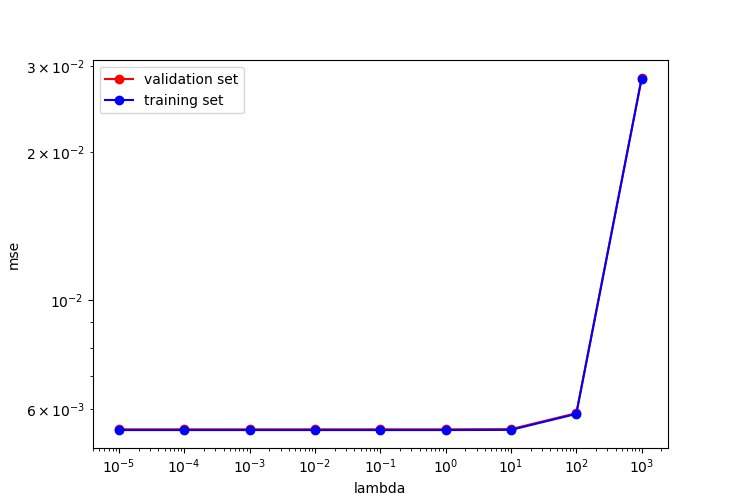
\includegraphics[width=0.5\textwidth]{LinearRegression.png}
\caption{Impact of Regularization Strength \(\lambda\) on Linear Regression Performance. }
\label{fig:image1}
\end{figure}

In Figure 1 we can see both curves overlap.\
We find that the mean square error in this case becomes bigger as we increase \(\lambda\).
So we will choose \(\lambda = 0\).

\section{Logistic Regression}

\subsection{Model Training}
Training involves converting labels to one-hot encoded vectors, initializing weights, and iteratively updating these weights to minimize the loss function. The update step at each iteration is guided by the learning rate and the gradient of the loss with respect to the weights. The process incorporates a softmax function to compute class probabilities and uses these probabilities to calculate the cross-entropy loss, thereby enabling the model to handle multiclass classification effectively. 

In the provided implementation of the logistic regression classifier, an essential optimization technique has been employed to enhance numerical stability:

\begin{lstlisting}
scores -= np.max(scores, axis = 1, 
                 keepdims = True)
\end{lstlisting}

This step adjusts the scores by subtracting the maximum score in each row before applying the exponential function. This operation ensures that the highest value in each set of scores is 0, significantly reducing the risk of exponential overflow, which can lead to NaN values during computation. Importantly, this optimization does not alter the outcome of the softmax function, as the subtraction of a constant value from all scores does not affect the relative differences between them.


\subsection{Hyperparameter Tuning}

\begin{figure}[htbp]
\centering
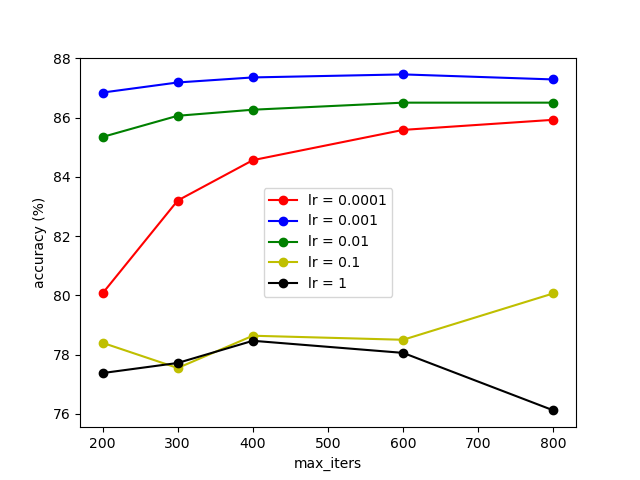
\includegraphics[width=0.5\textwidth]{LogisticRegression.png}
\caption{Impact of Learning Rate and Maximum Iterations on Model Accuracy (Validation Set). }
\label{fig:image2}
\end{figure} \

We ran KFold cross validation with \(K = 5\).
We clearly reach maximum accuracy with \(lr = 0.001\) and \(iters_{max} = 600\).

\section{K-Nearest Neighbors (KNN)}

\subsection{Model Training}
In regression tasks, the prediction is the weighted average of the labels of the \(k\) nearest neighbors. The weights are inversely proportional to the distances, giving closer neighbors more influence on the outcome. To ensure numerical stability and avoid division by zero, a small constant (\(1e-5\)) is added to the distances before computing the weights. This adjustment is crucial for maintaining the algorithm's robustness in scenarios where the distance between examples might be extremely small.

\begin{gather*}
\hat{y} = \frac{1}{\sum_{i=1}^{k} w_{NNi}} \sum_{i=1}^{k} w_{NNi}y_{NNi} \notag \\
w_{NNi} = \frac{1}{d(\mathbf{x}_{NNi}, \mathbf{x})}
\end{gather*}


Now for classification, the kNN algorithm identifies the \(k\) nearest neighbors and determines the output by selecting the most frequent label among them. This process inherently supports multi-class classification and is effective in capturing the local structure of the data. By relying on the majority vote.


\subsection{Hyperparameter Tuning}
\begin{figure}[htbp]
\centering
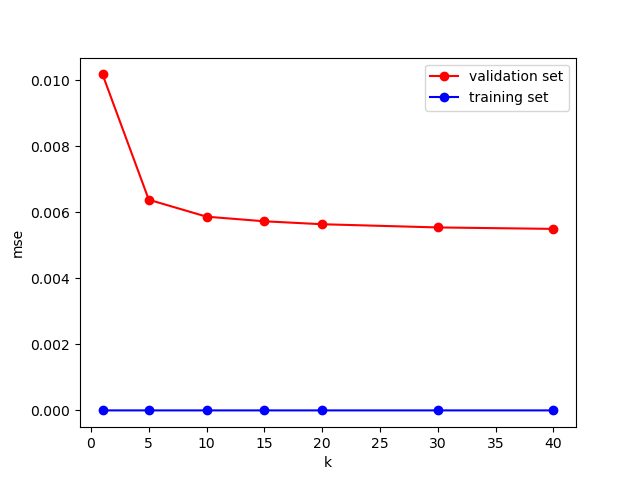
\includegraphics[width=0.5\textwidth]{KNNRegression.png}
\caption{Finding the Optimal k: Performance Analysis of kNN (regression). }
\label{fig:image3}
\end{figure} \

\begin{figure}[htbp]
\centering
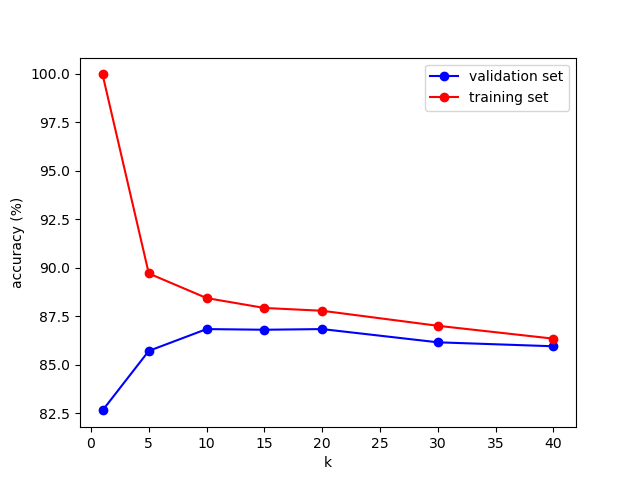
\includegraphics[width=0.5\textwidth]{KNNClassification.png}
\caption{Finding the Optimal k: Performance Analysis of kNN (classification). }
\label{fig:image4}
\end{figure} \

Clearly for regression \(k_{optimal} = 30\) and for classification \(k_{optimal} = 20\).

\section{Conclusion}
Finally this is the overall performance after the optimisation of the hyperparameters : 

\begin{table}[ht]
    \centering
    \begin{tabular}{cccc}
         -&  Linear Reg&  Logistic Reg& KNN\\
         Breed&  -&  86.2\%& 86.2\%\\
         Center&  0.005&  -& 0.005\\
    \end{tabular}
    \caption{Benchmark on Test Data}
    \label{tab:my_label}
\end{table}

Which outperforms the benchmark given in the Project Description.

\end{document}
